
\section{PIM\_01\_Praxisteil}

\subsection{Prozesse und Informationen}

\subsubsection{p1 Aufgabe S. 4}

Beispielprozess:\\
"`In der Regel wird ein Kunde dann den Kundendienst kontaktieren, wenn er ein subjektiv unl"osbares Problem mit einem Produkt oder einer Dienstleistung hat.
Die Erwartungen an den Kundendienst wird der Kunde mit seinen Erfahrungen abgleichen und bewusst oder unbewusst ein Urteil "uber seine Zufriedenheit oder Unzufriedenheit f"allen."'
\par
"`Auch wenn sich das Produkt in einem einwandfreien Zustand befindet und nur ein Bedienungsfehler vorliegt, dann der Kontakt von kunde und Unternehmen "uber Zufriedenheit und ggf. "uber Wiederholungsk"aufe entscheiden.
Ein Kunde wird dann zufrieden sein, wenn sein Problem durch eine effektive und schnelle Unterst"utzung eines Experten behoben wird.
Ein reibungsloser und einfacher Ablauf ist dabei ebenso wichtig wie die kompetente Beratug."'
\par
Erkl"aren Sie anhand deises Prozesses drei konkrete Ansatzpunkte, wie Informationsmanagement zur Prozessunterst"utzung genutzt werden kann.


\textbf{\#\#\# TODO \#\#\#}\\



\subsection{Infomrmationsmanagement}

\subsubsection{p1 Aufgabe S. 8}

F"ur die Entwicklung eines neuen Bibliotheksinformationssystems wird ein konzeptionelles Datenmodell in Form eines Entity-Relationship-Modells ben"otigt.
Folgender Sachverhalt ist abzubilden:\\
B"ucher werden von einem oder mehreren Autoren verfasst.
Jedes Buch ist eindeutig durch seine ISBN gekennzeichnet und erscheint genau in einem Verlag.
Ein Verlag ist durch Name und Ort eindeutig identifiziert.
Von jedem Buch existieren in der Bibliohek ein oder mehrere Exemplare, die von den Lesern ausgeliehen werden k"onnen.
Wird ein Exemplar ausgeliehen, so wird das R"uckgabedatum vermerkt.\\
Erstellen Sie bitte das zugeh"orige ERM.
Modellieren Sie auch die im Text angegebenen Attribute und erg"anzen Sie, wo notwendig, die jeweils identifizierenden Attribute.


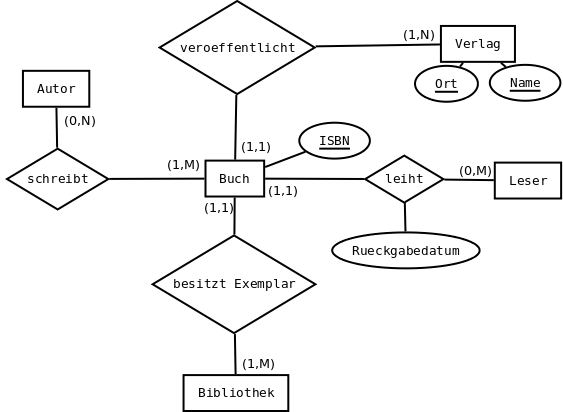
\includegraphics[scale=0.5]{./inc/p1_umlaufgabe}

\subsubsection{p1 Aufgabe S.24}
Ein wesentlicher Aspekt der relationalen Datenmodellierung ist die so genannte Normalisierung.\\
\noindent
a) Erl"autern Sie bitte, welches Ziel mit der Normalisierung verfolgt wird.
Welcher Pahse des Modellierungsprozesses ist die Normalisierung zuzuordnen?\\

\begin{quote}
Um der L"osch-, Einf"uge- und "Anderungs-Anomalie entgegen zu wirken m"ussen Tabellen normalisiert werden.
Das bedeutet, dass alle Redundanzen entfernt werden m"ussen.\\
Die Normalisierung l"asst sich der Feindatenmodellierung zuordnen.
\end{quote}

\noindent
b) Nennen und begr"unden Sie bitte, in welcher Normalform sich die folgende Tabelle befindet.\\

\begin{quote}
Die Tabelle "`Studenten\_zu\_Pr"ufungen"' ist in der \textbf{ersten Normalform}.
Sie ist in der ersten Normalform weil \textbf{jede Eigenschaft nur einen Eigenschaftswert} enth"alt.\\
Die Tabelle ist jedoch nicht in der zweiten Normalform, da Nicht-Schl"usselattribute abh"angig von einer echten Teilmenge der Schl"usselkandidaten ist.
\end{quote}

\noindent
c) "Uberf"uhren Sie die Tabelle aus Teilaufgabe b) bitte in die n"achsth"ohere Normalform.\\


\rowcolors{1}{LightGray}{White}
\begin{tabular}{ l l }
    \hline
    \rowcolor{LightSlateGrey}
    \textbf{Matrikelnummer} & \textbf{Studentname} \\
    111111                  & M"uller\\
    333333                  & Schmidt\\
\end{tabular}

\vspace{1cm}

\begin{tabular}{ l l }
    \hline
    \rowcolor{LightSlateGrey}
    \textbf{Pr"ufungsnummer}    & \textbf{Pr"ufungsname}\\
    6144                        & Prozess- und Informationsmanagement\\
    2377                        & E-Procurement\\
\end{tabular}

\vspace{1cm}

\begin{tabular}{ l l l }
    \hline
    \rowcolor{LightSlateGrey}
    \textbf{Matrikelnummer} & \textbf{Pr"ufungsnummer}  & \textbf{Note}\\
    111111                  & 6144                      & 1,0\\
    111111                  & 2377                      & 1,3\\
    333333                  & 6144                      & 2,0\\
\end{tabular}


